In the previous chapter we described how inference with the RNNG can be performed using a discriminative proposal model. We there used a discriminative RNNG; in this chapter we introduce an alternative. We introduce a novel neural Conditional Random Field (CRF) parser. The model is a CRF factored over labeled spans, and is an adaptation of the chart-based parser introduced in \citet{stern2017minimal} from margin-based training to global CRF training. The model is defined over normal form trees, but can deal with $n$-ary trees by binarization using a dummy label, and with unary chains by collapsing them to an atomic label.\footnote{\textit{Cf.} figure \ref{fig:trees-ptb} for this normalization process.}. Each of these labels are in turn treated as any other nonterminal label. This solution is adequate for the supervised training of the CRF and its application as parser, but does pose a challenge for the use of this model as proposal for the RNNG. The indifferent treatment of the dummy label causes derivational ambiguity, which in turn causes a subtle mismatch between the set of trees modelled by the CRF and the set of trees modelled by the RNNG. We discuss the effects of the derivational ambiguity and describe solutions at the end of the chapter.

In this chapter:
\begin{itemize}
  \item We present the model and describe how it is an adaptation into a CRF of the max-margin trained model of \citet{stern2017minimal}.
  \item We show how several inference problems of interest---parsing, sampling, and computing the entropy---can be solved exactly and efficiently by deriving specific instances of the inside and outside algorithms.
  \item We train the model in and show its effectiveness as discriminative parser: with the same number of parameters as the discriminative RNNG it achieves 90.04 F1, surpassing RNNG by more than 1 point F1.
  \item We use the trained model as a proposal distribution for the generative RNNG, and show that this does not affect the parsing accuracy, but does affect the perplexity, albeit negatively.
  \item We desribe the problems of the current formulation of the model as a proposal model for the RNNG, and we provide solutions. Preliminary results show that this solves the problem.
\end{itemize}

\section{Model}
   The model is a span-factored CRF that predicts scores for labeled spans over the sentence using neural networks, which then interact in a tree-structured dynamic program, giving a compact description of the probability distribution over all parses. This approach combines the efficient exact inference of chart-based parsing, the rich nonlinear features of neural networks, and the global training of a CRF. The factorization enables efficient exact inference alowing for exact decoding and global sampling while the neural features can be complex and can condition on the entire sentence.

    Let $x$ be a sentence, and $y$ a tree from $\yieldx$. We define a function $\Psi$ that assings nonnegative scores $\Psi(\x, \y)$ and let the probability of a tree be its globally normalized score
    \begin{align}
      \label{eq:crf-model}
      p(\y \mid \x) &= \frac{\Psi(\x, \y)}{Z(\x)},
    \end{align}
    where
    \begin{align*}
      Z(\x) = \sum_{ \y \in \yieldx } \Psi(\x, \y)
    \end{align*}
    is the normalizer, or partition function, that sums over the exponential number of trees availlable for $\x$.

    To allow efficient computation of the normalizer, we let the scoring function $\Psi$ factorize over the parts of $\y$. We consider a tree as a set of labeled spans $\y_c = (A, i, j)$, indicating that a label $A \in \Lambda$ spans the words $\langle x_{i+1}, \dots, \x_j \rangle$, and thus write $\y = \{ \y_c \}_{c=1}^C$. The value $\Psi(\x, \y)$ is then defined as the product
    \begin{align}
      \Psi(\x, \y) = \prod_{c=1}^C \psi(\x, \y_c),
    \end{align}
    where nonnegative potentials $\psi(\x, \y_c)$ score the parts. The function $\psi$ scores each labeled span $\y_c$ seperately, but conditional on the entire sentence.

    The above model is your typical constituency parsing CRF \citep{finkel2008crf,klein2015crf}. But where those models factorize trees over \textit{anchored rules}, our model the factorizes over \textit{labeled spans},\footnote{Compare table \ref{tab:spans-rules} for the different representations of a tree.} an approach first taken in \citet{stern2017minimal}. This factorization imposes an even stronger independence assumption than that imposed by factorizatin over anchored rules. By factorizing over labeled spans, the potential function $\psi$ has no access to information about the direct substructure under the node, such as the child nodes and their split point, and the function can thus rely less on the (local) tree structure and must thus rely more on the surface features of the input sentence. It will, however, greatly reduce the size of the state-space of the dynamic programs, speeding up training and inference, and the burden of the scoring function will be carried by a rich neural network parametrization. Together this will make the parser fast yet effective, which we will detail in section \ref{sect:inference} on inference.

\section{Parametrization}
  The scoring function $\psi$ is implemented with neural networks following \citet{stern2017minimal}. Again, let $\y_c$ denote a labeled span $(A, i, j)$ in a tree $\y$, and let $\psi(\x, \y_c) \geq 0$ be the score of that labeled span for sentence $\x$. These local potentials can only make minimal use of structural information but they can depend on the entire sentence. This suggest the use of bidirectional RNN encodings. Let $\fw_i$ and $\bw_i$ respectively be the vectors computed by a forward and backward RNN for the word in position $i$. The representation of the span $(i, j)$ is the concatenation of the difference between the vectors on the endpoints of the span:
  \begin{align}
    \label{eq:span-feature}
    \vecs_{ij} = [\fw_j - \fw_i; \bw_i - \bw_j].
  \end{align}
  The vector $\vecs_{ij}$ represents the words $x_i^j$, and equation \ref{eq:span-feature} is illustrated in figure \ref{fig:span-feature}. The scores for each label in that position are computed from this vector using a feedforward network with output dimension $\reals^{\lvert \Lambda \rvert}$, and the score of label $A$ is given by the index corresponding to it:
  \begin{align}
    \label{eq:potential-function}
    \log \psi(\x, \y_c) = [ \ff( \vecs_{ij} ) ]_{A},
  \end{align}
  where we pretend that $A$ doubles as an index. This architecture is rightly called minimal, but it works surprisingly well: \citet{stern2017minimal} also experiment with more elaborate functions based on concatenation of vectors (a strict superset of the minus approach) and biaffine scoring (inspired by \citet{dozat2016deep}), but these functions improve marginally, if they do at all.

  \begin{figure}
    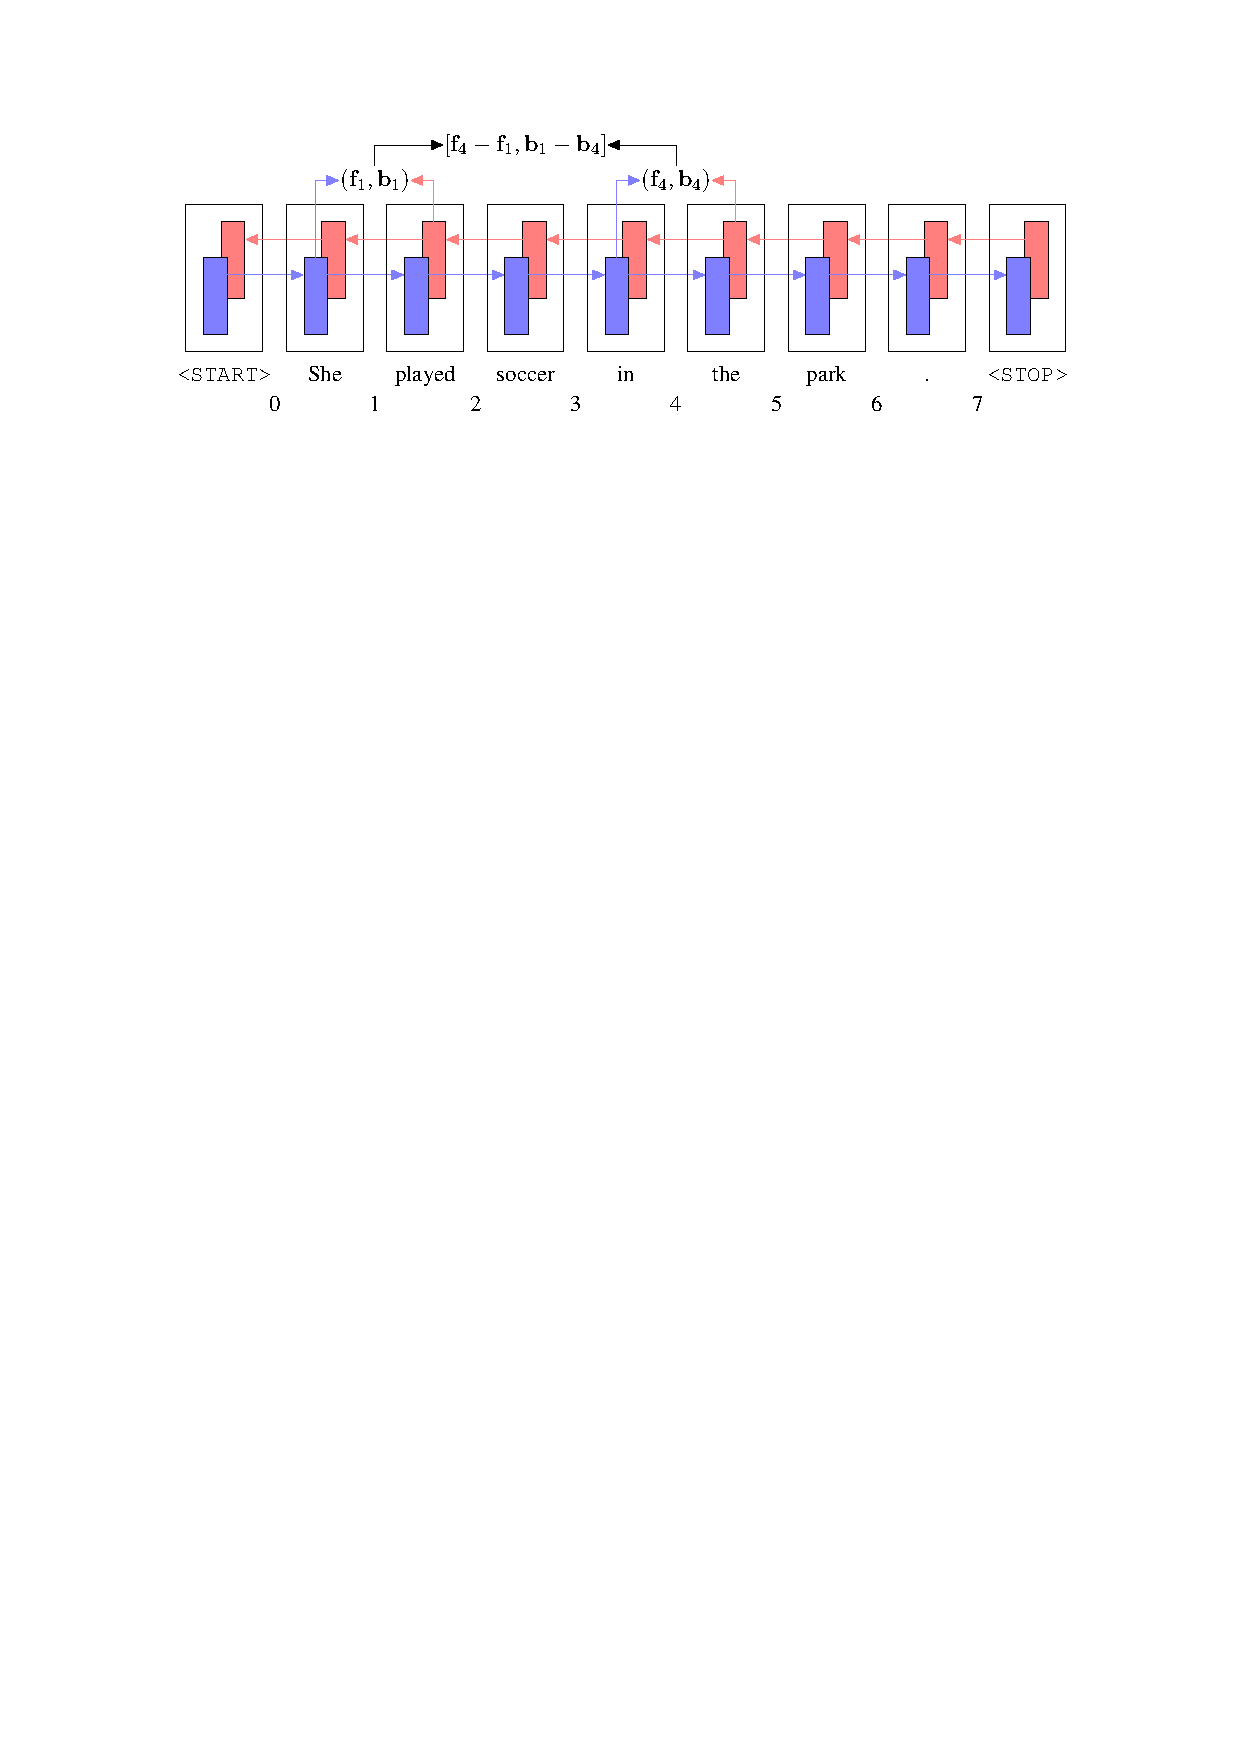
\includegraphics[width=\textwidth]{span-encoding.pdf}
    \caption{Representation for the span $(1, 4)$ computed from RNN encodings. Figure taken from \citet{stern2018analyis}.}
    \label{fig:span-feature}
  \end{figure}

\section{Inference}
  \label{sect:inference}
  Because our model is span-factored it allows efficient inference. In this section we describe efficient solutions to four related problems:
  \begin{itemize}
    \item Compute the normalizer $Z(\x) = \sum_{ \y \in \yieldx } \prod_{ c=1 }^{ C } \psi( \x, \y_c )$.
    \item Find the best parse $\hat{ \y } = \arg \max_{\y } p(\y  \mid \x)$
    \item Sample a tree $Y \sim P(Y \mid X = x)$.
    \item Compute the entropy $\entropy(Y \mid X = x)$ over parses for $\x$.
  \end{itemize}
  These problems can be solved by instances of the \textit{inside algorithm} and \textit{outside algorithm} \citep{baker1979trainable} with differentent semirings, an insight we take from semiring parsing \citep{goodman1999semiring}. In the following derivations we will make use of the notion of a \textit{weighted hypergraph} as a compact representation of all parses and their scores \citep{gallo1993directed,klein2004parsing}, and use some of the ideas and notation of \textit{semiring parsing} \citep{goodman1999semiring,eisner2009semirings}. First we describe the structure of the parse forest specified by our CRF parser, and then derive the particular form of the inside and outside recursions for this hypergraph from the general formulations. We refer the reader to appendix \ref{A3-crf} for background on these ideas, and the introduction of the notation.

  \subsection{Weighted parse forest}
    The the CRF parser defines a hypergraph $G = (\mathcal{V}, \mathcal{E})$ with the following structure. We treat the dummy label $\varnothing \in \Lambda$ as any other label, unless we explictly indicate otherwise.

    The set $\mathcal{V}$ is defined relative to the sentence $\x$, and contains the invidual words of a sentence $\x$, together with all possible labeled spans over that sentence:
    \begin{align*}
      \mathcal{V} = \Big\{ \x_i \; \Big\vert \; 1 \leq i \leq n \Big\} \cup \Big\{ (A, i, j) \; \Big\vert \; A \in \Lambda, 0 \leq i < j \leq n \Big\} \cup \Big\{ (S^{\dagger}, 0, n) \Big\},
    \end{align*}
    where $(S^{\dagger}, 0, n)$ is a designated root node. The dependence on $x$ can be made explicit by writing $\mathcal{V}(x)$.

    The set of hyperedges $\mathcal{E} \subseteq 2^{\mathcal{V}} \times \mathcal{V}$ specifies all the ways that adjacent constituents can be combined to form a larger constituent, under a particular grammar. The edges connect sets of nodes at the \textit{tail} with a singel node at the \textit{head}. Because we (implicitly) assume a normal form grammar that contains \textit{all} possible productions, the set of hyperedges is particularly regular: the set $\mathcal{E}$ contains all edges that connect nodes $(B, i, k)$ and $(C, k, j)$ at the tail with $(A, i, j)$ at the head for all $0 \leq i < k < j \leq n$, all edges that connect $\x_i$ to $(A, i, i+1)$, and all labels can appear in the top node, with the exception of the dummy label $\varnothing$:
    \begin{align*}
      \mathcal{E}
        &= \Bigg\{ \Big\langle \Big\{ (B, i, k), (C, k, j) \Big\},  (A, i, j) \Big\rangle \; \Bigg\vert \; A, B, C \in \Lambda, \; 0 \leq i < k < j \leq n \Bigg\}  \\
        &\quad\cup \Bigg\{ \Big\langle \{ \x_i \}, (A, i-1, i) \Big\rangle \; \Bigg\vert \; A \in \Lambda, \; 1 \leq i \leq n \Bigg\}  \\
        &\quad\cup \Bigg\{ \Big\langle \{ (A, 0, n) \}, (S^{\dagger}, 0, n) \Big\rangle \; \Bigg\vert \; A \in \Lambda \setminus \{ \varnothing \} \Bigg\}
    \end{align*}
    The three kind of edges that make up $\mathcal{E}$ are illustrated in figure \ref{fig:crf-edges}. A tree is a set of nodes $y \subseteq \mathcal{V}(x)$, and the parse forest a set of trees $\yieldx \subseteq 2^{\mathcal{V}(x)}$.

    \begin{figure}[h]
      \center
      \begin{tikzpicture}[scale=.6]
        % \documentclass[11pt]{article}
% \usepackage{tikz}
% \usepackage{amsmath,amssymb,amsfonts}
%
% \usetikzlibrary{arrows,calc}
%
% \begin{document}

% \tikzstyle{every node}=[circle, draw, inner sep=0pt, minimum size=7mm]
%
% \tikzstyle{every node}=[circle, draw, inner sep=0pt, minimum size=11mm, node distance =1 cm and 1cm ]

% \begin{tikzpicture}

\node(a){$x_i$} ;
\node(b) at ($(a)+(4.5,0)$){$B_{i}^{k}$} ;
\node(c) at ($(b)+(3,0)$){$C_{k}^{j}$} ;
\node(d) at ($(c)+(4.5,0)$){$A_{0}^{n}$} ;

\node(A1) at ($(a)+(0,3)$){$A_{i-1}^{i}$} ;
\node(A2) at ($(b)+(1.5,3)$){$A_{i}^{j}$} ;
\node(S) at ($(d)+(0,3)$){$S^{\dagger n}_{0}$} ;

\draw[->] (a) to [in=-90,out=90](A1);

\draw[->] (b) to [in=-90,out=90](A2);
\draw[->] (c) to [in=-90,out=90](A2);

\draw[->] (d) to [in=-90,out=90](S);

% \end{tikzpicture}
%
% \end{document}

      \end{tikzpicture}
      \caption{The edge-types making up the hypergraph. The edges are instatiated for all $A, B, C \in \Lambda$ and all $0 \leq i < j \leq n$. Only for the rightmost edge holds the restriction $A \neq \varnothing$, to ensure that the dummy label cannot be the top node.}
      \label{fig:crf-edges}
    \end{figure}

    We connect a semiring $\mathcal{K}$ to the hypergraph by defining the weight function as $\omega: \mathcal{E} \to \mathbb{K}$, and by accumulating the weights with its binary operations. The function $\omega$ that assigns weights to the edges is given by either the function $\psi$ or $(\log \circ \, \psi)$, depending on the semiring used. Because of this association, the function $\omega$ has a very particular property: the function effectively depends only on the \textit{head} of the edge. Given edges $e = \langle \{ u, w \}, v \rangle$ and $e' =  \langle \{ u', w' \}, v \rangle$ for $u \neq u'$ and $w \neq w'$, their weights are equal: $\omega(e) = \omega(e')$. For this reason we write $\omega(v)$ instead.\footnote{Thus implicitly defining $\omega: \mathcal{V} \to \mathbb{K}$.} This fact will allow us to greatly simplify the recursions that follow. Additionally, this means that instead of computing independent scores for each of the $O(n^3 \vert\Lambda\rvert^3)$ edges, we only need to compute scores for the $O(n^2 \vert\Lambda\rvert)$ vertices. For a scoring function like a neural network, for which computation can be relatively expensive, this will make a significant difference.

   With this structure in place, we are ready to derive the form of the inference algorithm particular to this structure.

  \subsection{Inside recursion}
    The inside recursion computes quantities $\alpha(A,i,j)$ for all labels $A \in \Lambda$ and all spans $0 \leq i < j \leq n$ with respect to a semiring. What the quantity represents depends on the semiring used. In this section we derive the inside recursion specific to our hypergraph from the general result given.

    Let $\mathcal{K}$ be some semiring with binary operations $\oplus$ and $\otimes$ and identity elements $\bar{0}$ and $\bar{1}$. The inside recursion is given by the formula \citep{goodman1999semiring}
    \begin{align*}
      \alpha(v) =
        \begin{cases}
          \bar{1}  &  \mbox{if } I(v) = \varnothing,  \\
          \displaystyle\bigoplus_{e \in I(v)} \omega(e) \otimes \displaystyle\bigotimes_{u \in T(e)} \alpha(u)  & \mbox{otherwise.}
        \end{cases}
    \end{align*}
    Here $I(v) \subseteq E$ is the set of edges incoming at node $v$, and $T(e) \subseteq V$ is the set of nodes in the tail of edge $e$.

    At a node $v = (A, i, i+1)$ that spans one word $x_i$, the inside value is just the weight of the single edge incoming from that word:
    \begin{align}
        \label{eq:inside-base}
        \alpha(A, i, i+1) = \omega(A, i, i+1) \otimes \alpha(x_i) = \omega(A, i, i+1),
    \end{align}
    for $A \in \Lambda$, for all $0 \leq i < n$. We used the fact that $\alpha(x_i) = \bar{1}$, which follows from the fact that there are no arrows incoming at $\x_i$.

    For a general node $\alpha(A, i, j)$, $j > i + 1$, we observe that all the incoming edges have at the tail the nodes $(B, i, k)$ and $(C, k, j)$, for all $B, C \in \Lambda$ and $i < k < j$. The sum over edges thus reduces to independent sums over $B$, $C$, and $k$, and the product over the inside values at the tail reduces to the product of values $\alpha(B, i, k)$ and $\alpha(C, k, j)$. The form of $\omega$ allows us to rewrite this greatly as
    \begin{align}
      \label{eq:inside}
      \alpha(A, i, j)
        &= \bigoplus_{B \in \Lambda} \bigoplus_{C \in \Lambda} \bigoplus_{k=i+1}^{j-1} \omega(A, i, j) \otimes \alpha(B,i,k) \otimes \alpha(C,k,j) \nonumber \\
        &= \omega(A, i, j) \otimes \bigoplus_{k=i+1}^{j-1} \bigoplus_{B \in \Lambda} \alpha(B,i,k) \otimes \bigoplus_{C \in \Lambda} \alpha(C,k,j) \nonumber \\
        &= \omega(A, i, j) \otimes \bigoplus_{k=i+1}^{j-1} \sigma(i,k) \otimes \sigma(k,j),
    \end{align}
    where we have introduced the notational abbreviation
    \begin{align*}
        \sigma(i,j) &= \bigoplus_{A \in \Lambda} \alpha(A,i,j).
    \end{align*}
    Looking at \ref{eq:inside} we can see the marginalized values $\sigma(i, j)$ are all that are needed for the recursion. This suggest simplifying the recursion even further as
    \begin{align}
      \label{eq:inside-simplified}
      \sigma(i, j)
        &= \bigoplus_{A \in \Lambda} \alpha(A,i,j) \nonumber \\
        &= \Bigg[ \bigoplus_{A \in \Lambda} \omega(A, i, j) \Bigg] \otimes \Bigg[\bigoplus_{k=i+1}^{j-1} \sigma(i,k) \otimes  \sigma(k,j) \Bigg],
    \end{align}
    where we put explicit brackets to emphasize that independence of the subproblems of labeling and splitting.

    These values can be computed by visiting the nodes of the parse forest in topological order. This order ensures that the quantities in the tail of an edge will have been computed when the value at the node at the head is at turn. Given the highly regular form of the parse forest, this order boils down to something quite simple: the nodes are visited by increasing width of the span; the order in which the starting-points are visited does not matter because these nodes are not connected among each other.\footnote{\textit{Cf.} figure \ref{fig:hypergraph} in appendix \ref{A3-crf}: the width of the span determines the vertical level of the node in the parse forest; for a fixed width, the label and startpoint are all unconnected along this vertical level, and thus independent.}. We choose to visit the starting points from left to right, that is, from 0 to $n$.

  \subsection{Outside recursion}
    The outside algorithm computes the quantities $\beta(A,i,j)$ for all labels $A \in \Lambda$ and all spans $0 \leq i < j \leq n$. The general recursion is given by:
    \begin{align*}
      \beta(v) =
        \begin{cases}
          \bar{1}  & \mbox{if } O(v) = \varnothing, \\
          \displaystyle\bigoplus_{e \in O(v)} \omega(e) \otimes \beta(H(e)) \otimes \displaystyle\bigotimes_{ \substack{ w \in T(e) \\ w \neq u } } \alpha(w)  & \mbox{otherwise.}
        \end{cases}
    \end{align*}
    Here, $O(v) \subseteq E$ is the set of edges outgoing from $v$, $\ie$ the edges for which $v$ is in the tail, and define $H(e) \in V$ as the node at the head of edge $e$.

    The only node without outgoing edges is the root node, and thus
    \begin{align*}
      \beta(S^{\dagger}, 0, n) = \bar{1}.
    \end{align*}
    To compute $\beta(A, i, j)$ in the general case we need to sum over all outgoing edges. These come in two kinds: either $(A, i, j)$ combines with $(C, j, k)$ to form constituent $(B, i, k)$; or $(A, i, j)$ combines with $(C, k, i)$ to form constituent $(B, k, j)$. This corresponds to the following expression, that we can simplify by making use of the properties of $\omega$:
    \begin{align*}
      \beta(A, i, j)
        &= \bigoplus_{B \in \Lambda} \bigoplus_{C \in \Lambda} \bigoplus_{k=1}^{i-1} \omega(B, k, j) \otimes \alpha(C, k, i) \otimes \beta(B, k, j) \\
          &\qquad \oplus \bigoplus_{B \in \Lambda} \bigoplus_{C \in \Lambda} \bigoplus_{k=j+1}^{n} \omega(B, i, k) \otimes \beta(B, i, k) \otimes \alpha(C, j, k) \\
        &=  \bigoplus_{k=1}^{i-1}  \Bigg[ \bigoplus_{B \in \Lambda} \omega(B, k, j)  \otimes \beta(B, k, j) \Bigg] \otimes \Bigg[ \bigoplus_{C \in \Lambda} \alpha(C, k, i) \Bigg] \\
          &\qquad \oplus \bigoplus_{k=j+1}^{n}  \Bigg[ \bigoplus_{B \in \Lambda}  \omega(B, i, k) \otimes \beta(B, i, k) \Bigg] \otimes  \Bigg[  \bigoplus_{C \in \Lambda} \alpha(C, j, k) \Bigg] \\
        &=  \bigoplus_{k=1}^{i-1}  \sigma'(k, j) \otimes \sigma(k, i) \oplus \bigoplus_{k=j+1}^{n} \sigma'(i, k) \otimes  \sigma(j, k) \\
    \end{align*}
    where
    \begin{align*}
        \sigma(i, j) &= \bigoplus_{A \in \Lambda} \alpha(A, i, j),  \\
        \sigma'(i, j) &= \bigoplus_{A \in \Lambda} \omega(A, i, j) \beta(A, i, j).
    \end{align*}

    These values can be computed by visiting the nodes of the parse forest in \textit{reverse} topological order, exactly the opposite of the inside recursion. This order ensures that the quantities in the head of an edge will have been computed when the values in the tail are at turn. Again, this this order boils down to something quite simple: the nodes are visited based by decreasing width of their span, and again the order of the start-points are free.

  \subsection{Solutions}
    Equiped with the two recursions and a handful of semirings we can provide the solutions promised at the outset of this section.

    \paragraph{Normalizer}
      When we intantiate the inside recursion with the real semiring, the value of $\alpha$ at the root is the normalizer:
      \begin{align*}
        \alpha(\text{S}^{\dagger}, 0, n) = Z(\x),
      \end{align*}
      and when we instantiate the inside recursion with the log-real semiring we obtain the log-normalizer
      \begin{align*}
        \alpha(\text{S}^{\dagger}, 0, n) = \log Z(\x).
      \end{align*}

    \paragraph{Parse}
      To find the viterbi tree $\hat{ \y } = \arg \max_{ \y } p(\y  \mid \x)$ and its probability $p(\hat{\y} \mid \x)$ we use the Viterbi semirings ($\cf$ examples \ref{ex:vit-weight} and \ref{ex:vit-derivation} in appendix \ref{A3-crf}). We take equation \ref{eq:inside-simplified} and use the Viterbi semiring operations to derive that the value of the best subtree spanning words $i$ to $j$ is given by
      \begin{align}
        \label{eq:viterbi-score}
        \sigma(i,j)
          &= \max_{A} [ \log \psi(A, i, j) ] + \max_{k} [\sigma(i,k) + \sigma(k,j)].
      \end{align}
      The value $\log \Psi(\x, \hat{\y})$ is then given by $\sigma(0, n)$, and  can be normalized with to give the probability
      \begin{align}
        \log p(\hat{y} \mid x) = \sigma(0, n) - \log Z(x).
      \end{align}
      The best label and splitpoint $\hat{A}$ and $\hat{k}$ for the span $(i, j)$ are obtained by using the argmax:
      \begin{align}
        \label{eq:viterbi-tree}
        \hat{A} &= \argmax_{ A  } \log \psi(A, i, j)  \\
        \hat{k} &= \argmax_{ k } \sigma(i, k) + \sigma(k, j),
      \end{align}
      and the best tree $\hat{y}$ is found by following back from the root down to the leaves the best splits and labels.

    \paragraph{Sample}
      Unbiased samples from the model can be obtained by recursively sampling incoming edges, starting at the root node $(S^{\dagger}, 0, n)$, ending at the word nodes. The probability of an edge is proportional to the weight of all the trees under that edge. This is precicely what is represented by the inside value $\alpha$ computed in the real-semiring. At node $v = (A, i, j)$ the probability of edge $e = \langle \{ u, w \}, v \rangle$, with $u = (B, i, k)$ and $w = (C, k, j)$, is thus
      \begin{align}
        \label{eq:sample}
        P(E = e \mid V = v)
          &= \frac{\omega(e) \otimes \bigotimes_{u \in T(e)} \alpha(u)}{\alpha(v)}  \nonumber  \\
          &= \frac{\psi(A, i, j) \, \alpha(B, i, k) \, \alpha(C, k, j)}{\alpha(A, i, j)}.
      \end{align}
      Once an edge is sampled, the process is repeated at the nodes in the tail of that edge. We stop when we reach the nodes that span individual words. The sampled edges together then are guaranteed to form a tree. From a compuational point of view, this sampling is very efficient: the scores for the labeled spans need to be computed only once, followed by a single run of the inside and outside algorithm. Beyond this point, no costly computation is required. In our case, where the scores are predicted by a neural network, this means that we need to perfom just a single forward pass. Compare this with a sequential model such as the discriminative RNNG, where each sample requires an separate forward pass.

    \paragraph{Entropy}
      % To compute the entropy $H(Y \mid X = x)$ we need to first introduce the notion of the \textit{maginal probablity} of a node. The marginal of a node $v = (A, i, j)$ in a hypergraph is the probability that it occurs in a tree $\y$ for the sentence $\x$ as governed by the distribution $p$ that we defined on it. Let $V$ be a random variable with the hypergraph nodes $\mathcal{V}(x)$ as sample space, and define
      % \begin{align}
      %   P(V = v \mid X = \x)
      %     &\defeq \expect_Y[ \indicator_{ \{ v \in Y \} } ]  \nonumber \\
      %     &= \sum_{ \y \in \yieldx } p(\y \mid \x) \indicator_{ \{ v \in y \} }.
      % \end{align}
      %
      % The marginals can be computed from the inside and outside values computed in the real semiring as
      % \begin{align}
      %   P(V = v \mid X = \x) = \frac{\alpha(A, i, j) \, \beta(A, i, j)}{Z(\x)},
      % \end{align}
      % a result from \citep{goodman1999semiring}.\footnote{This can also be seen by noting that the product of $\alpha(A, i, j)$ and $\beta(A, i, j)$ is the sum over all trees that contain the node $v$, and $Z(\x)$ the sum over all trees in general.} The entropy can then be written as an expectation with respect to these marginals:
      % \begin{align}
      %   H(Y \mid X = x)
      %     &= - \sum_{ \y \in \yieldx } p(\y \mid \x) \log p(\y \mid \x)  \nonumber \\
      %     &= \log Z(\x) - \sum_{ \y \in \yieldx } p(\y \mid \x) \sum_{v \in \y} \log \psi(\x, v)  \nonumber \\
      %     &= \log Z(\x) - \sum_{ \y \in \yieldx } p(\y \mid \x) \sum_{ v \in \mathcal{V}(x) } \indicator_{ \{ v \in y \} } \log \psi(\x, v)  \nonumber \\
      %     &= \log Z(\x) - \sum_{ v \in \mathcal{V}(x) } \log \psi(\x, v)  \sum_{ \y \in \yieldx } \indicator_{ \{ v \in y \} } p(\y \mid \x)  \nonumber \\
      %     &= \log Z(\x) - \sum_{ v \in \mathcal{V}(x) } \log \psi(\x, v)  P(V = v \mid X = \x)  \nonumber \\
      %     &=  \log Z(\x) - \expect_V [ \log \psi(\x, V) ].
      % \end{align}
      To compute the entropy $\entropy(Y \mid X = x)$ we need to first introduce the notion of a \textit{node maginal}. The marginal of a node $v = (A, i, j)$ in a hypergraph is the probability that it occurs in a tree $\y$ for the sentence $\x$, according to the probability distribution $p$ over trees. The node marginal $\mu(v)$ is defined as the expectation
      \begin{align}
        \label{eq:node-marginal}
        \mu(v)
          &\defeq \expect[ \indicator( v \in Y ) ]  \nonumber \\
          &= \sum_{ \y \in \yieldx } p(\y \mid \x) \indicator( v \in y ).
      \end{align}
      This can be computed from the inside and outside values computed in the real semiring as
      \begin{align}
        \mu(v) = \frac{\alpha(A, i, j) \, \beta(A, i, j)}{Z(\x)},
      \end{align}
      a result from \citep{goodman1999semiring}. This can also be seen by noting that the product of $\alpha(A, i, j)$ and $\beta(A, i, j)$ is the sum over all trees that contain the node $v$, and $Z(\x)$ the sum over all trees in general.

      The entropy, then can then be written in terms of these marginals:
      \begin{align}
        \label{eq:crf-entropy}
        \entropy(Y \mid X = x)
          &= - \sum_{ \y \in \yieldx } p(\y \mid \x) \log p(\y \mid \x)  \nonumber \\
          &= \log Z(\x) - \sum_{ \y \in \yieldx } p(\y \mid \x) \sum_{v \in \y} \log \psi(\x, v)  \nonumber \\
          &= \log Z(\x) - \sum_{ \y \in \yieldx } p(\y \mid \x) \sum_{ v \in \mathcal{V}(x) } \indicator( v \in y ) \log \psi(\x, v)  \nonumber \\
          &= \log Z(\x) - \sum_{ v \in \mathcal{V}(x) } \log \psi(\x, v)  \sum_{ \y \in \yieldx } \indicator( v \in y ) p(\y \mid \x)  \nonumber \\
          &= \log Z(\x) - \sum_{ v \in \mathcal{V}(x) } \log \psi(\x, v) \mu(v)
      \end{align}

\section{Training}
  The CRF is trained to maximize the log likelihood of a labeled dataset $\dataset$ of pairs $(\x, \y)$
  \begin{align*}
    \mathcal{L}(\theta)
      &= \sum_{(\x, \y) \in \dataset} \log \ptheta(\y \mid \x)
  \end{align*}
  with respect to the model parameters $\theta$.

    Writing out the objective for a single example as
    \begin{align*}
      \log \ptheta(\y \mid \x) = \log \Psi(\x, \y) - \log Z(x)
    \end{align*}
    reveals that the maximization of this value decomposes as two separate optimizationproblems: to maximize the log-score of the example tree $\log \Psi(\x, \y)$, whilst minimizing the log of the total weight of the parse forest $\log Z(x)$. The solution is thus to move probability mass onto the gold tree $\y$, and away from \textit{all other trees}. Because the log-score of the tree decomposes as a sum of log-scores of the nodes that it comprises, the objective is effectively to \textit{increase} the scores of the labeled spans that make up the gold tree, and \textit{decrease} the scores of all other labeled spans not observed. Another effect of this factorization into spans is that such an update increases not only the probability of the gold tree, but the probability of all trees that share substantial substructure. It is in this precise sense that we mean that the model learns about all substructures.

    We rely on automatic differentiation to compute the derivatives, but note that in principle it is possible to efficiently combine the computation of the inside and outside values with their derivatives, a fact demonstrated in \citep{eisner2009semirings} and \citep{eisner2016backprop}, and implemented in \citep{kim2017structured}.\footnote{Amongst others, we do not take because it would require us to implement custom gradient computations in our toolkit of choice Dynet \cite{neubig2017dynet}, which is far from trivial.}

    It is fruitful to see how our global objective differs from the margin-based objective in \citep{stern2017minimal}. The margin-based objective is to maximize the difference, or `margin', between the score of the gold tree and the highest scoring, incorrect tree. Given a sentence $\x$ the model computes the predicted tree $\hat{y}$. If the predicted tree equals the gold tree, $\hat{y} = \y$, then no changes to the model parameters are made. Otherwise, the model parameters are updated to maximize the difference between their scores
    \begin{align*}
      \log \Psi(\x, \y) - \log \Psi(\x, \hat{\y}),
    \end{align*}
    maximizing the score of the correct tree, and minimizing the score of the predicted tree.\footnote{The full objective reported in the paper is minimizing the hinge loss $\max \Big(0, 1 - \log \Psi(\x, \y) + \log \Psi(\x, \hat{\y}) \Big)$, and the above is what the actual implementation comes down to. Note that Viterbi ensures that for all $\y$, $\log \Psi(\x, \hat{\y}) \geq \log \Psi(\x, \y)$.} This objective shows a striking similarity with our CRF objective, with one very particular difference. The goal is still to maximize the score of the gold tree. But the minimization that in the CRF objective concerns all possible trees through $Z(x)$, in this objective concerns just the single tree $\hat{\y}$ that was incorrectly predicted. The scores of all other nodes not observed in either tree are not affected directly.

  % \subsection{Speed and complexity}
  %   The model is slow. Here we will describe how slow it is, and what can be done about it.
  %   \begin{itemize}
  %     \item During training the computation time is dominated by two computations: the forward pass with the neural networks that obtains the node scores, and the time complexity of the inside algorithm. The complexity of the and how it depends on both label size and sentence length
  %     \item Describe how slow the model is to train of CPU (use Lisa times): around 7 hours per epoch, so around 15 days for convergence (around 50 epochs).
  %     \item Describe how we can speed up linearly by pruning the labelset: we can remove 70\% of labels while keeping 98\% of the training sentences. These labels are mostly very rare unary chains. The speedup we get from this is linear!
  %     \item Our model is X times slower than the model of \citet{stern2017minimal}. This difference bust be in the inside algorithm. The inside algorithm used by us and the viterbi algorithm used by \citet{stern2017minimal} have the same structure and time complexity. The difference must be in the computation graph built by either computation. The viterbi algorithm builds a sparse computation graph, connecting only nodes that are in a single tree, whereas the computation graph built by the inside algorithm is dense with all trees.
  %   \end{itemize}

\section{Experiments}
  This section reports the results of the experiments performed with the CRF parser. We first train the model on the Penn Treebank and show that it is a strong parser. The CRF obtains a higher F1 than the discriminative RNNG when trained with the same number of parameters; an even higher F1 is obtained when or models is trained with the same hyperparameters as the model in \citet{stern2017minimal}. We then use the CRF as an alternative proposal model for the generative RNNG and perform analyses similar to those in chapter \ref{03-rnng}. This use of the CRF leads to some theoretical challenges. We note these, but discuss them in detail in the next section.

  \subsection{Setup}
    We train two versions of the model on the Penn Treebank: a small version and a large version. The smaller model allows us to compare the CRF parser to the discriminative RNNG, while the larger model allows us to compare it to the parser of \citet{stern2017minimal}. The smaller model has dimensions to match the number of parameters in the discriminative RNNG from chapter \ref{03-rnng} and is trained in the same way. For the larger model we follow the dimensions and optimization details of \citet{stern2017minimal}.

    For both models the embeddings are of dimension 100, and the LSTMs have 2 layers. For the smaller model the dimension of forward and backward the LSTM is 128, and the feedforward network has one hidden layer with dimension 256. For the larger model we follow the hyperparameters of \citet{stern2017minimal}: the LSTMs have dimesion 250, just as the feedforward network. Given these dimensions, the total number of parameters in the small model is around 0.75M and around 2.5M for the large model (the exact numbers are in table \ref{tab:num-params}). The small CRF is comparable in size with the discriminative RNNG (around 0.8M parameters) and less than a third in size of the larger model. The smaller model is optimized exactly as the discriminative RNNG: SGD with learning rate 0.1, and dropout of 0.2. For the larger model we use Adam \citep{kingma2014adam} with 0.001 and dropout of 0.4, exactly following \citet{stern2017minimal}.

  \subsection{Results}
    The evaluation setup is the same as in the previous chapter. We train 10 models from different random seeds, and we report mean and standard deviations, as well as scores of the best model selected by development F1.

    % \begin{table}[h]
% \center
% \footnotesize
%   \begin{tabular}{l|c|c|c|c}
%       & Small & Large & \citet{stern2017minimal} & \citet{stern2018analyis} word-only  \\ \hline
%     F1  & $89.94 \pm	0.12$ \quad (90.04) & $90.31 \pm 0.15$ \quad (90.43) &  -- \quad (91.79) &  -- \quad (91.44)
%   \end{tabular}
%   \caption{F1 scores for the CRF.}
%   \label{tab:disc-fscores}
% \end{table}

\begin{table}[h]
  \center
  \footnotesize
  \begin{tabular}{l|c|c|c}
      & Small & Large & \citet{stern2017minimal} \\ \hline
    F1  & $89.94 \pm	0.12$ \quad (90.04) & $90.31 \pm 0.15$ \quad (90.43) &  -- \quad (91.79)
  \end{tabular}
  \caption{F1 scores for the CRF.}
  \label{tab:disc-fscores}
\end{table}


    The results are shown in \ref{tab:crf-fscores}. Both models perform well, achieving on average 89.94 F1 for the smaller model and 90.31 F1 for the larger model. The small difference in F1 between the two is surprising given difference in size and optimization, and speaks for the relative robustness of our model with respect to these choices. Our best small CRF (90.04 F1) surpasses the best discriminative RNNG (88.58) by almost 2.5 F1, but our best large CRF (90.43) performs below the model of \citet{stern2017minimal} (91.79). Just as for the RNNG, we believe this can be attributed to the absence of tags. However, we can note that---in case this is true---the negative impact is much greater for the RNNG (around 3.1 F1 lower) than in the CRF (around 1.4 F1 lower).

  \subsection{Proposal distribution}
    We have introduced the CRF parser as an alternative proposal model for the generative RNNG, and we now evaluate the CRF in this role. We repeat the same inference procedure as in chapter \ref{03-rnng}: we sample 100 trees from the small CRF with the highest development F1, and use these to evaluate the same generative RNNG as before. The results are shown in tables \ref{tab:gen-fscores-crf} (F1) and \ref{tab:gen-perplexities-crf} (perplexity), and include the previous results for comparison.

    \begin{table}[h]
\center
\footnotesize
  \begin{tabular}{l|c|c|c}
      Proposals & Our RNNG & CRF & \citet{dyer2016rnng} &  \\ \hline
      Ours  & $91.07 \pm	0.1 \quad (91.12)$  &  $91.02 \pm 0.05 \quad (91.04)$ &  $93.32 \pm 0.1 \quad (93.32)$  \\
      \citet{dyer2016rnng}  & -- & -- & -- \quad (93.3)
  \end{tabular}
  \caption{F1 scores for the generative RNNG, for different proposal models. The first column is with proposals from our discriminative RNNG, the final column is with the proposals used by \citet{dyer2016rnng} to evaluate, availlable at \url{https://github.com/clab/rnng}.}
  \label{tab:gen-fscores}
\end{table}


    \begin{table}[h]
\center
\footnotesize
  \begin{tabular}{l|c|c|c}
       & RNNG & CRF & \citet{dyer2016rnng}  \\ \hline
      Our RNNG & $108.76 \pm	1.52 \quad (107.43)$  &  $117.79 \pm 2.1 \quad (116.28)$ &  $107.80 \pm 1.59 \quad (106.45)$  \\
      \citet{dyer2016rnng}  & -- & -- & -- \quad (105.2)  \\
      \citet{kuncoro2017syntax}  & -- & -- & -- \quad (100.9)
  \end{tabular}
  \caption{Perplexity on the PTB of the generative RNNG, for different proposal models.}
  \label{tab:gen-perplexities-crf}
\end{table}


    The results for the F1 are virtually the same. Although the CRF is the better parser by F1, both are equivalent with respect to generative RNNG. On average, however, because the discriminative RNNG proposals performs better on the selected model. A real difference can be observed in the perplexity, with a difference of over 9 nats in favour of the RNNG.

  \subsection{Analysis}

    We perform the same analyses of the approximate inference as in chapter \ref{03-rnng}, this time with the CRF as proposal model. The results of the experiment on aproximate inference are shown in figure \ref{fig:samples-fscores-crf} (F1) and \ref{fig:samples-perplexities-crf} (perplexity), where they are compared to the results of the annealed RNNG. With respect to parsing F1, the CRF is the better choice when using few samples, but for this difference disappears for larger number of samples.

    Figure \ref{fig:samples-entropy-crf} shows the estimation of the conditional entropy, now including the results for the CRF. The estimates of the CRF converge to the true conditional entropy, which can be computed exactly and equals 2.84.\footnote{To be precise, the values $\entropy(Y \mid X = x)$ can be computed exactly, the value $\entropy(Y \mid X)$ is still estimated by a mean over the test set.} Furthermore we can note that the conditional entropy of the CRF is higher than that of the discriminative RNNG when not annealed. This could indicate that the CRF maintains a higher number of alternative parses per sentence on average than the RNNG. Another plausible explanation is that the higher entropy is caused by the derivational ambiguity: the higher entropy reflects that each tree has multiple derivations. We address this possibility in the next section.

    % \begin{figure}[h]
    %   \center
    % 	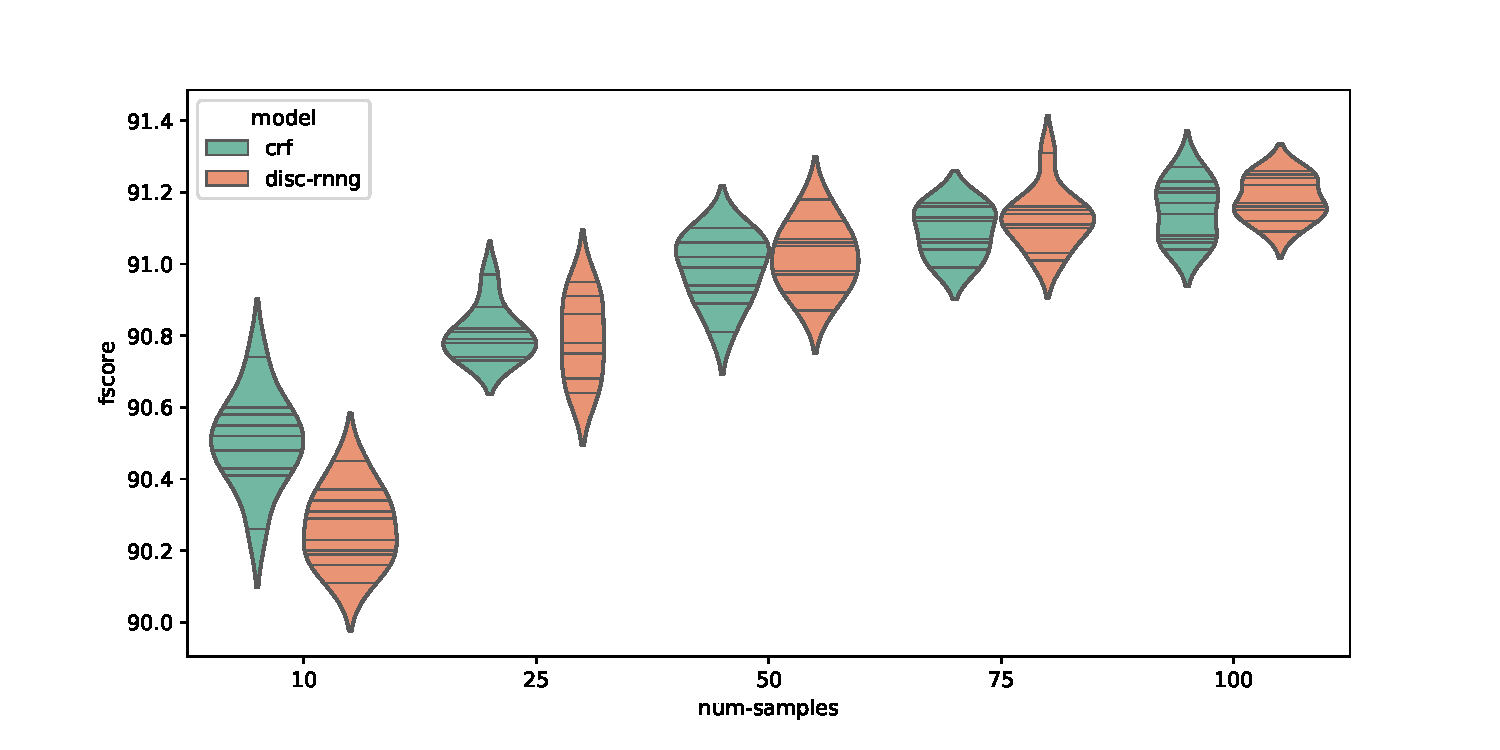
\includegraphics[width=0.9\textwidth]{sample-experiment/fscore/crf_disc_08.pdf}
    % \caption{F1 estimated with increasing number of samples, with CRF and discriminative RNNG annealed with $\alpha=0.8$, for 10 independent repetitions.}
    % \label{fig:samples-fscores-crf}
    % \end{figure}
    %
    % \begin{figure}[h]
    %   \center
    % 	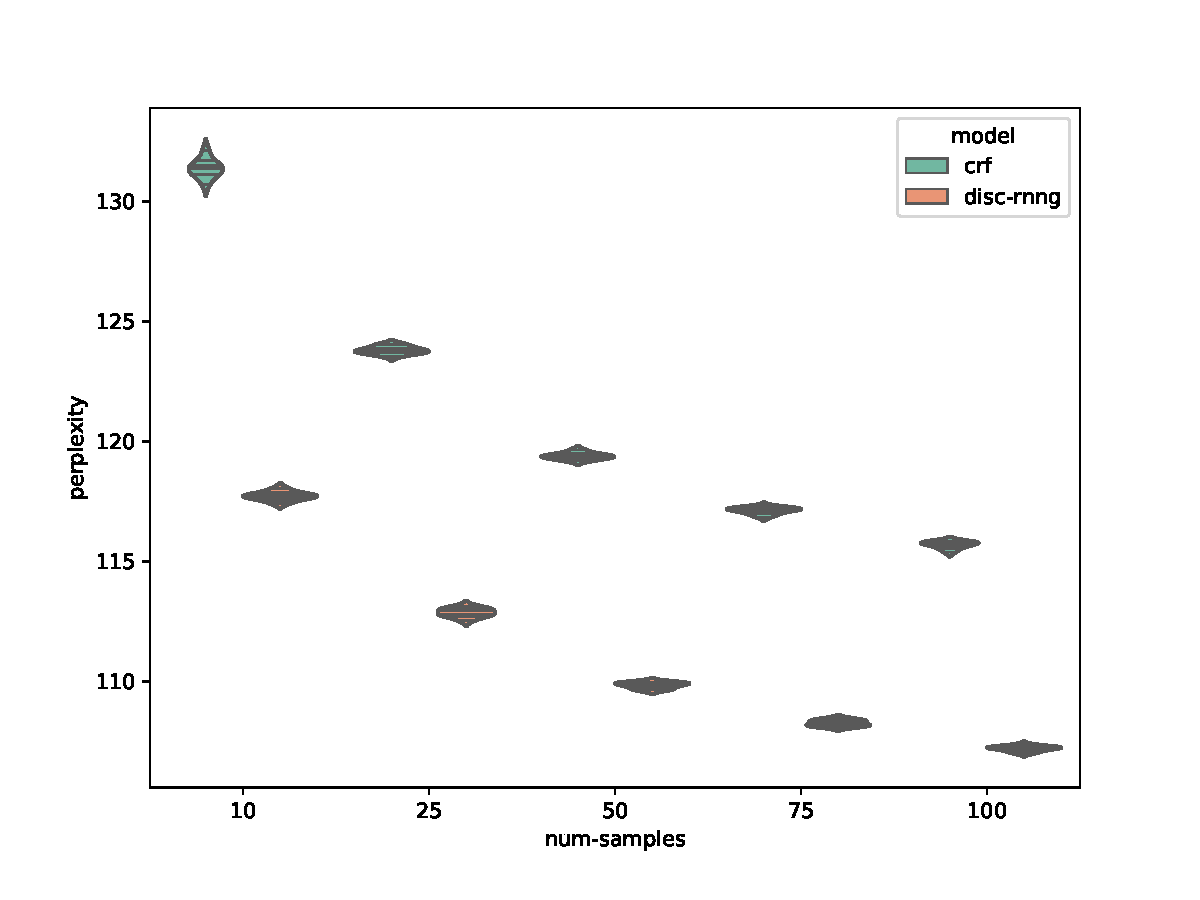
\includegraphics[width=0.7\textwidth]{sample-experiment/ppl/crf_disc08.pdf}
    % \caption{Perplexity estimated with increasing number of samples, with CRF and discriminative RNNG annealed with $\alpha=0.8$, for 10 independent repetitions.}
    % \label{fig:samples-perplexities-crf}
    % \end{figure}
    %
    % \begin{figure}[h]
    %   \center
    %   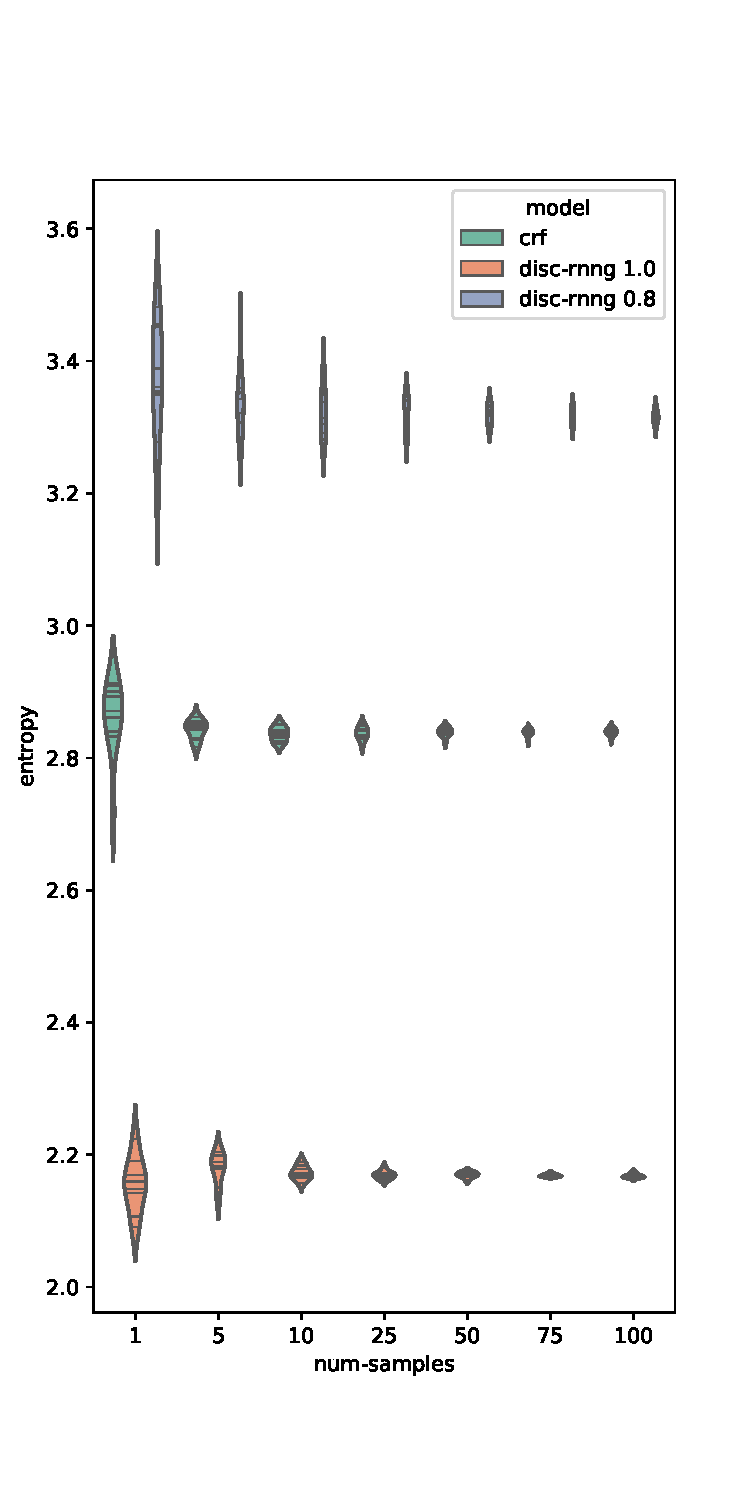
\includegraphics[width=0.4\textwidth]{sample-experiment/entropy/all.pdf}
    % \caption{Conditional entropy estimated with increasing number of samples.}
    % \label{fig:samples-entropy-crf}
    % \end{figure}

    \begin{figure}[h]
      \center
    	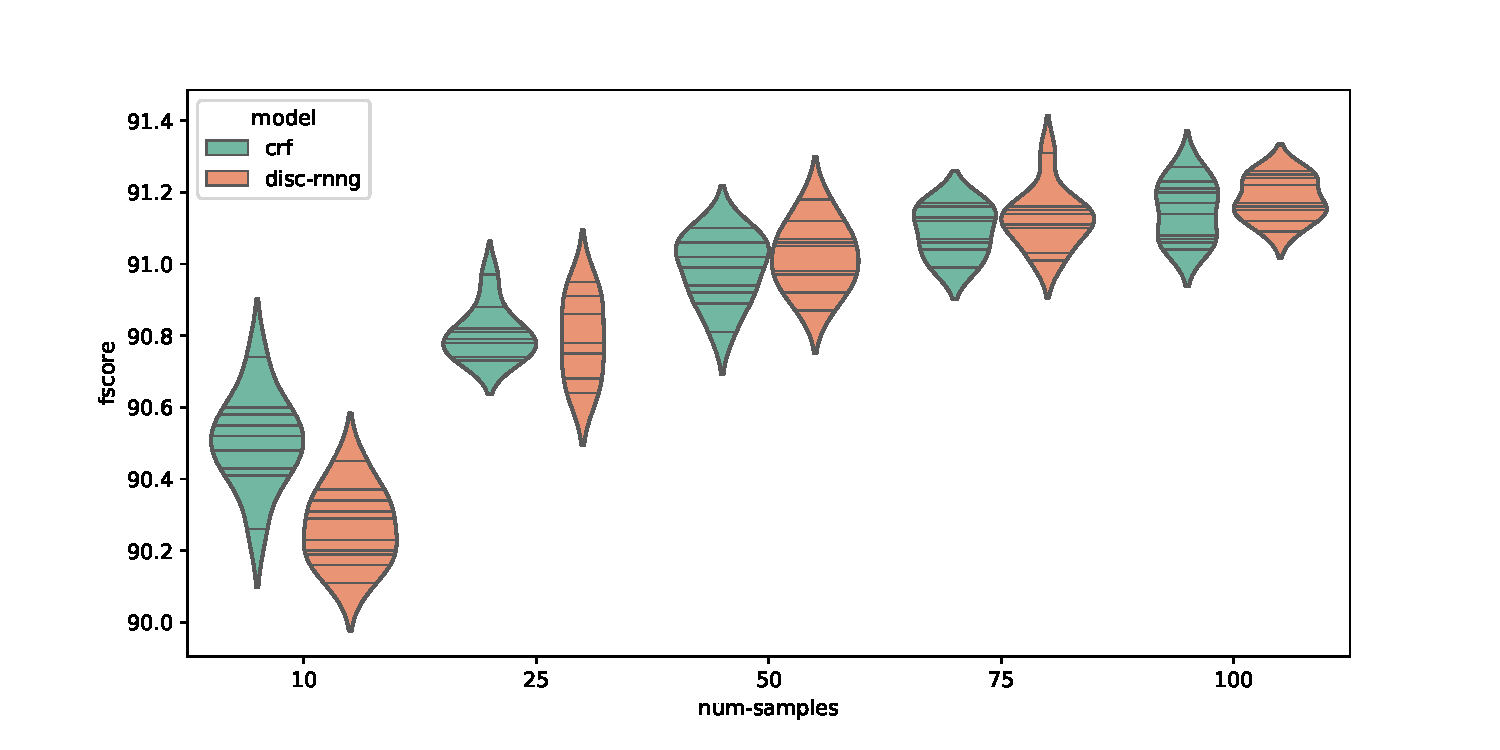
\includegraphics[width=0.9\textwidth]{sample-experiment/fscore/crf_disc_08.pdf}
      \caption{F1 estimated with increasing number of samples, with CRF and discriminative RNNG annealed with $\alpha=0.8$, for 10 independent repetitions.}
      \label{fig:samples-fscores-crf}
    \end{figure}

    \newgeometry{top=5mm, bottom=5mm}  % enables full page view
    \begin{figure}[h]
      \center
    	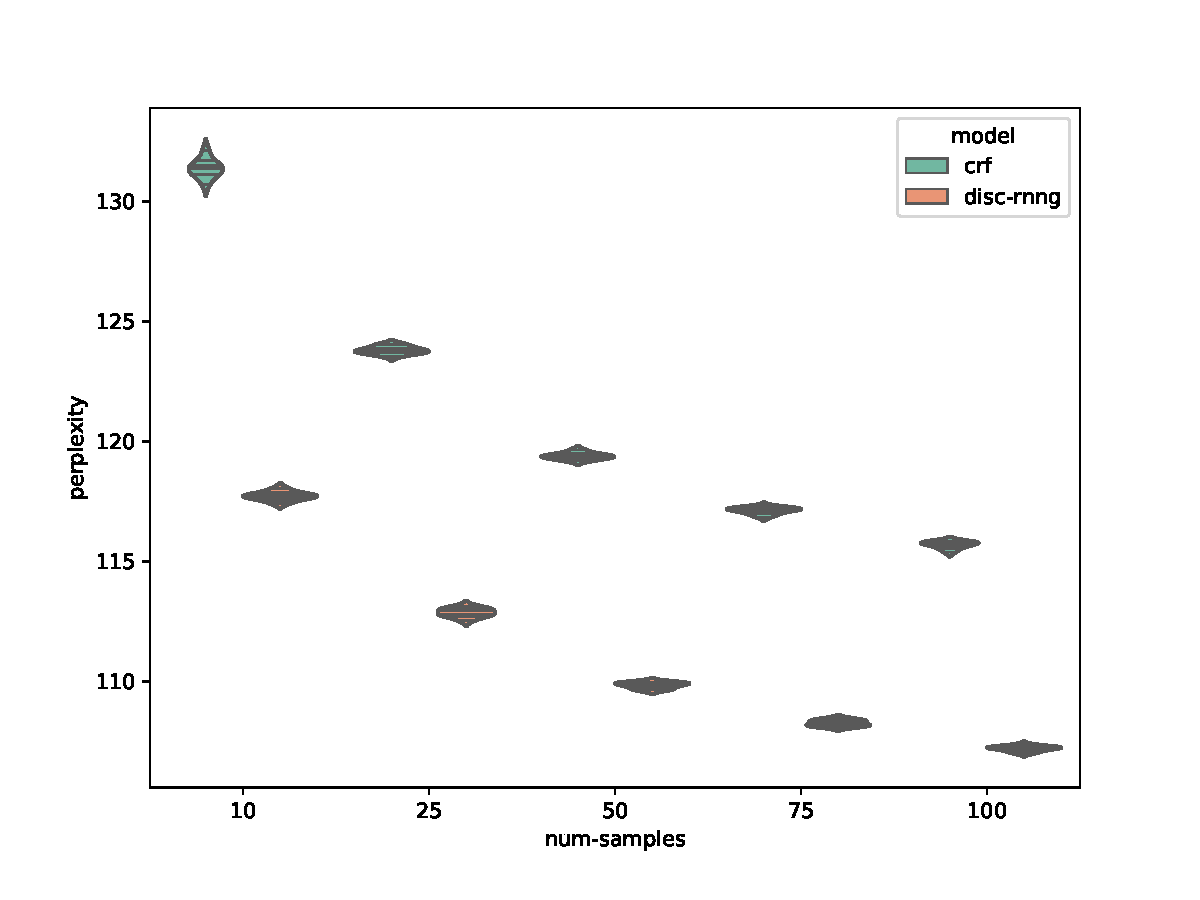
\includegraphics[width=0.8\textwidth]{sample-experiment/ppl/crf_disc08.pdf}
      \caption{Perplexity estimated with increasing number of samples, with CRF and discriminative RNNG annealed with $\alpha=0.8$, for 10 independent repetitions.}
      \label{fig:samples-perplexities-crf}

      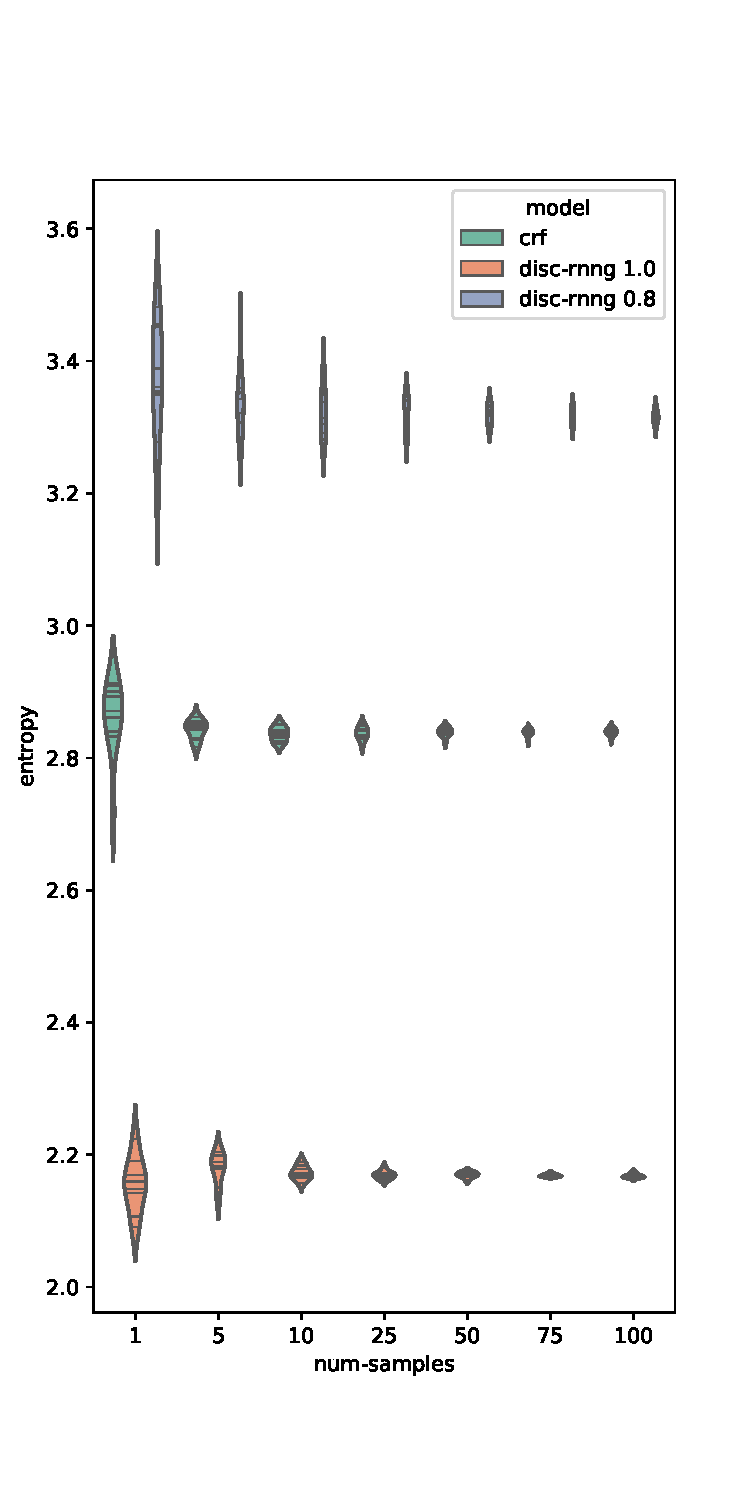
\includegraphics[width=0.5\textwidth]{sample-experiment/entropy/all.pdf}
      \caption{Conditional entropy estimated with increasing number of samples.}
      \label{fig:samples-entropy-crf}
    \end{figure}
    \restoregeometry

\section{Trees and derivations}
  The use of the CRF as a proposal distribution brings to light a subtle issue: by our choice of binarization we have introduced derivational ambiguity, and this affects the approximate marginalization. In this section we will describe the issue, which we characterize as the difference between the binary \textit{derivations} and the \textit{trees} they collapse to. We analyze the impact of this on the approximate marginalization, and then propose solutions. We will return to this difference in chapter \ref{05-semisupervised}, where the computation of the entropy plays a central role.

  \subsection{Derivational ambiguity}
    The way our CRF deals with binarization and its inverse introduces the problem derivational ambiguity: many binary derivation $d$ modelled by the CRF as distinct map to the same tree $y$ when the dummy node is collapsed. In other words: we map a treebank tree to a single normal form derivation, but many normal form derivations map to a that treebank tree. For example, the two normal form trees in \ref{fig:normal-form-trees} both collapse to the same tree when dummy labels $\varnothing$ are collapsed:
    \begin{center}
      (S (NP The other hungry cat) (VP meows) .).
    \end{center}
    However, when going the other way---applying the normal form transformation to the above tree---we always obtain the left tree, and never the right tree. Let $f: \yieldx \to \mathcal{D}(x)$ be the transformation that we defined that produces normal form trees from treebank trees, and let $g: \mathcal{D}(x) \to \yieldx$ be the transformation that takes a normal form tree and collapses the dummy nodes. Then $f$ is a bijection, but $g$ is not: for any tree $y$ the preimage of $g$ is the set of derivations $g^{-1}( y ) = D \subseteq \mathcal{D}(x)$ that collapse to the same tree. And generally, $\lvert D \rvert > 1$. This is the issue at hand: going from derivations to trees causes derivational ambiguity.

    \begin{figure}[h]
      \begin{subfigure}[b]{0.5\textwidth}
        \center
        \begin{tikzpicture}[scale=.8]
          \Tree [.S
        [.NP
          [.$\varnothing$ The ]
          [.$\varnothing$ [.$\varnothing$ other ] [.$\varnothing$ [.$\varnothing$ hungry ] [.$\varnothing$ cat ] ] ] ]
        [.$\varnothing$ [.VP meows ] [.$\varnothing$ . ] ] ]

        \end{tikzpicture}
    	\end{subfigure}
    	\begin{subfigure}[b]{0.5\textwidth}
        \center
        \begin{tikzpicture}[scale=.8]
          \Tree [.S
        [.NP
          [.$\varnothing$ The ]
          [.$\varnothing$ [.$\varnothing$ [.$\varnothing$ other ] [.$\varnothing$ hungry ] ] [.$\varnothing$ cat ] ] ]
        [.$\varnothing$ [.VP meows ] [.$\varnothing$ . ] ] ]

        \end{tikzpicture}
    	\end{subfigure}
      \caption{Two normal form derivations that collapse to the same tree.}
      \label{fig:normal-form-trees}
    \end{figure}

  \subsection{Consequences}
    The direct consequence of the derivational ambiguity is that our CRF actually defines a distribution over $\mathcal{D}(x)$, and over $\yieldx$ only through by summing over the derivations that collapse to it. Let $\y$ be a general tree such as is modelled by the RNNG. Our CRF assigns probabilities to all $d \in f^{-1}(y)$ and defines a distribution over $\yieldx$ through
    \begin{align*}
      p(y \mid x) = \sum_{d \in f^{-1}(y)} p(d \mid x).
    \end{align*}
    As a consequence $p(d \mid x) \leq p(y \mid x)$ for all of the derivations $d$ that collapse to $y$. This has three direct consequences:
    \begin{itemize}
      \item We overestimate the marginal probability in the importance sampling:
        \begin{align*}
          \frac{1}{K}\sum_{i=1}^K  \frac{\ptheta( \x, \y^{(i)} )}{\qlambda(d^{(i)} \mid \x)}
            &\geq \frac{1}{K}\sum_{i=1}^K  \frac{\ptheta( \x, \y^{(i)} )}{\sum_{d \in f^{-1}(y^{(i)})} \qlambda(d \mid \x)}  \\
            &= \frac{1}{K}\sum_{i=1}^K  \frac{\ptheta( \x, \y^{(i)} )}{\qlambda(\y^{(i)} \mid \x)}  \\
            &\approx \expect_{q} \bigg[\frac{\ptheta(\x,\y )}{\qlambda(\y \mid \x)} \bigg] = \ptheta(\x).
        \end{align*}
      \item Viterbi returns the best derivation, not necessarily the best tree. In other words, if $\hat{d} = \argmax_d p(d \mid \x)$ then $g(\hat{d}) \neq \argmax_y p(\y \mid \x)$ in general. This is a situation similar to decoding in latent variable PCFGs \citep{petrov2006learning}, which is known to be intractable \citep{sima2002computational}.
      \item The entropy is over derivations instead over trees, and it is not clear how one relates to the other.
    \end{itemize}
    The derivational ambiguity does not affect the samples: the probability that we draw $y$ is precisely the probability that we draw any $d$ in $f^{-1}(y)$.

  \subsection{Solutions}
    We propose two solutions to this problem:
    \begin{enumerate}
      \item We can dispense with the dummy label altogether, and instead alter our CRF so that it can deal directly with $m$-ary trees, for any order $m$. This means that we add all hyperedges with more than 2 children. The general formulation of the inside and outside recursions remain unaltered, but the specific form becomes less efficient because we now need to deal with a sum over all possible partitions of the span under a node.
      \item We keep the dummy label, but prune the hyperforest to only contain derivations that are reachable by the normal form transformation. This means that we assign probability zero to all trees that do not correspond to the cannonical normal form that we commited to by choosing the transformation. Because this transformation is very regular, we can easily incorporate this pruning in the inside and outside algorithms.
    \end{enumerate}

    We now describe either solution, starting with the solution of making the CRF deal directly with $m$-ary trees.

  \subsection{Unrestricted parse forest}
    One solution, as noted, is to make the parse-forest deal with $m$-ary trees directly. This requires that for each noterminal node, we add incoming edges that contain more than two children in the tail. This needs to be done for each permissible number of children---determined by the width of the span---and for all possible partitions of that size of the span.

    More formally, let $(A,i,j)$ be a node with $i + 1 < j$, so that it can expand to other noterminal nodes. Then let $i = k_0 < k_1 < k_2 < \cdots < k_m = j$ be a partition of the discrete interval $[i, j]$ into $m$ subspans. Since a span must have a width of at least 1, $m$ can be at most $j-i$ Letting $B_1, \dots, B_m$ be labels for those subspans we can form an edge that connects the set
    \begin{align*}
      \Big\{ (B_1, k_0, k_1), (B_2, k_1, k_2), \dots, (B_m, k_{n-1}, k_m) \Big\}
    \end{align*}
    at the tail to the node $(A, i, j)$ at the head. Adding \textit{all} such nodes to the parse forest for each $m$ will allow us to deal with trees of unrestricted arity directly.

    The generality of the semiring formulations of the inside and outside algorithms, allows us to seamlesly apply them to this new parse forest. If we let $v = (A, i, j)$ such that $I(v) \neq \varnothing$ we can derive the inside value $\alpha(v)$ as
    \begin{align*}
      \alpha(v)
        &= \displaystyle\bigoplus_{e \in I(v)} \omega(e) \otimes \displaystyle\bigotimes_{u \in T(e)} \alpha(u)  \\
        &= \displaystyle\bigoplus_{m = 2}^{j - i} \displaystyle\bigoplus_{k_0 < k_1 < \cdots < k_m} \displaystyle\bigoplus_{B_1 \in \Lambda} \cdots \displaystyle\bigoplus_{B_m \in \Lambda} \omega(A, i, j) \otimes \displaystyle\bigotimes_{l=1}^n \alpha(B_l, k_{l-1}, k_l) \\
        &= \omega(A, i, j) \otimes \displaystyle\bigoplus_{m = 2}^{j - i} \displaystyle\bigoplus_{k_0 < k_1 < \cdots < k_m} \displaystyle\bigotimes_{l=1}^n \displaystyle\bigoplus_{B \in \Lambda} \alpha(B, k_{l-1}, k_l) \\
        &= \omega(A, i, j) \otimes \displaystyle\bigoplus_{m = 2}^{j - i} \displaystyle\bigoplus_{k_0 < k_1 < \cdots < k_m} \displaystyle\bigotimes_{l=1}^n \sigma(k_{l-1}, k_l), \\
    \end{align*}
    where logic that allows us write
    \begin{align*}
      \displaystyle\bigoplus_{B_1 \in \Lambda} \cdots \displaystyle\bigoplus_{B_m \in \Lambda} \displaystyle\bigotimes_{l=1}^n \alpha(B_l, k_{l-1}, k_l) = \displaystyle\bigotimes_{l=1}^n \displaystyle\bigoplus_{B \in \Lambda} \alpha(B, k_{l-1}, k_l)
    \end{align*}
    is the same as in the binary case, but generalized to $m$ terms.

    For the outside value $\beta(v)$ we can follow a similar derivation. Let
    \begin{align*}
      0 \leq k_0 < \cdots < k_a = i < j = k_{a+1} < \cdots < k_m \leq n
    \end{align*}
    be a partition of the discrete interval $[k_0, k_m]$ into $m$ pieces, one of which is $[i, j]$, namely the interval $[k_a, k_{a+1}]$. This partition represents one way in wich the interval $[i, j]$ can be completed with $m-1$ other intervals into an interval $[k_0, k_m]$. With this in place, we can derive the outside recursion as
    \begin{align*}
      \beta(v)
        &= \displaystyle\bigoplus_{e \in O(v)} \omega(w) \otimes \beta(H(e)) \otimes \displaystyle\bigotimes_{ \substack{ w \in T(e) \\ w \neq u } } \alpha(w) \\
        &= \displaystyle\bigoplus_{m = 2}^{n - j + i} \displaystyle\bigoplus_{k_0=0}^{i-1} \displaystyle\bigoplus_{k_m = j}^{n} \displaystyle\bigoplus_{k_0 < \cdots < k_a < k_{a+1} < \cdots < k_m} \displaystyle\bigoplus_{B \in \Lambda}  \\
          &\qquad\qquad \omega(A, i, j) \otimes \beta(B, k_0, k_m) \otimes \displaystyle\bigotimes_{ \substack{1 \leq l \leq n \\ l \neq a } } \displaystyle\bigotimes_{C \in \Lambda} \alpha(C, k_{l-1}, k_l) \\
        &= \displaystyle\bigoplus_{m = 2}^{n - j + i} \displaystyle\bigoplus_{k_0=0}^{i-1} \displaystyle\bigoplus_{k_m = j}^{n} \displaystyle\bigoplus_{k_0 < \cdots < k_a < k_{a+1} < \cdots < k_m}  \\
          &\qquad\qquad \displaystyle\bigoplus_{B \in \Lambda} \omega(B, i, j) \otimes \beta(B, k_0, k_m) \otimes \displaystyle\bigotimes_{ \substack{1 \leq l \leq n \\ l \neq a } } \displaystyle\bigotimes_{C \in \Lambda} \alpha(C, k_{l-1}, k_l)  \\
        &= \displaystyle\bigoplus_{m = 2}^{n - j + i} \displaystyle\bigoplus_{k_0=0}^{i-1} \displaystyle\bigoplus_{k_m = j}^{n} \displaystyle\bigoplus_{k_0 < \cdots < k_a < k_{a+1} < \cdots < k_m} \sigma'(k_0, k_m) \otimes \displaystyle\bigotimes_{ \substack{1 \leq l \leq n \\ l \neq a } } \sigma(k_{l-1}, k_l).
    \end{align*}

    The above two recursions show that this approach is challenging, despite its elegance. Enumerating the sets of partitions is in itself already a nontrivial task.

  \subsection{Pruned parse forest}
    Another solution is to prune the parse forest: to keep only those trees that can be obtained by the normal form transformation. Going back to the example at the beginning of the example, this solution asks us to assign probability zero to the right tree, the tree that we cannot obtain by the normal form transformation. Since the transformation that we apply is very regular, we can easily characterize the set of trees that are impossible to derive. In fact, it boils down to one characteristic: a node can have the label $\varnothing$ only when \textit{either} that node spans a single word \textit{or} that node is the right child of its parent node.\footnote{We binarize \textit{rightwards}, thus introducting the dummy labels in that position, and can only ever introduce the dummy label in the left child position when it spans a single word.} That means we should remove from the parse forest all edges of the form illustrated in figure \ref{fig:illegal-edges}. By this same reasoning we conclude that the parse forest should also be rid of all nodes of the form $(\varnothing, 0, j)$ for $j > 1$, which cannot occur in any tree obtained with our transformation.

    \begin{figure}[h]
      \center
      \begin{tikzpicture}[scale=.6]
        % \documentclass[11pt]{article}
% \usepackage{tikz}
% \usepackage{amsmath,amssymb,amsfonts}
%
% \usetikzlibrary{arrows,calc}
%
% \begin{document}

% \tikzstyle{every node}=[circle, draw, inner sep=0pt, minimum size=7mm]
%
% \tikzstyle{every node}=[circle, draw, inner sep=0pt, minimum size=11mm, node distance =1 cm and 1cm ]

% \begin{tikzpicture}

\node(b){$\varnothing_{i}^k$} ;
% \node(b){$\varnothing_{i,k}$} ;
\node(c) at ($(b)+(2,0)$){$B_{k}^j$} ;
% \node(c) at ($(b)+(2,0)$){$B_{k,j}$} ;

\node(A2) at ($(b)+(1,3)$){$A_{i}^j$} ;
% \node(A2) at ($(b)+(1,3)$){$A_{i,j}$} ;

\draw[->] (b) to [in=-90,out=90](A2);
\draw[->] (c) to [in=-90,out=90](A2);

% \end{tikzpicture}
%
% \end{document}

      \end{tikzpicture}
      \caption{Edges in the parse forest that produce the derivational ambiguity, whenever $k > i+1$.}
      \label{fig:illegal-edges}
    \end{figure}

    With this characterization in hand, we can alter the recursions, starting with the inside algorithm.
    \begin{align}
      \label{eq:inside-pruned}
      \alpha(A, i, j)
        &= \displaystyle\bigoplus_{B \in \Lambda} \displaystyle\bigoplus_{C \in \Lambda} \omega(A, i, j) \otimes \alpha(B,i,i+1) \otimes \alpha(C,i+1,j) \nonumber \\
          &\qquad\oplus \displaystyle\bigoplus_{B \in \Lambda \setminus \{ \varnothing \} } \displaystyle\bigoplus_{C \in \Lambda} \displaystyle\bigoplus_{k=i+2}^{j-1} \omega(A, i, j) \otimes \alpha(B,i,k) \otimes \alpha(C,k,j) \nonumber \\
        &= \omega(A, i, j) \otimes  \Bigg[ \displaystyle\bigoplus_{B \in \Lambda}\alpha(B,i,i+1) \otimes  \displaystyle\bigoplus_{C \in \Lambda} \alpha(C,i+1,j)  \nonumber \\
          &\qquad\oplus \displaystyle\bigoplus_{k=i+2}^{j-1} \displaystyle\bigoplus_{B \in \Lambda \setminus \{ \varnothing \} } \alpha(B,i,k) \otimes \displaystyle\bigoplus_{C \in \Lambda} \alpha(C,k,j)  \Bigg]  \nonumber \\
        &= \omega(A, i, j) \otimes \Bigg[ \sigma(i,i+1) \otimes \sigma(i+1,j) \oplus \displaystyle\bigoplus_{k=i+2}^{j-1} \tilde{\sigma}(i,k) \otimes \sigma(k,j) \Bigg]
    \end{align}
    where
    \begin{align}
      \tilde{\sigma}(i,k) = \displaystyle\bigoplus_{B \in \Lambda \setminus \{ \varnothing \} } \alpha(A, i, k).
    \end{align}

    For the outside algorithm we need to split cases: the outside algorithm sums over ways to complete a labeled span into a larger labeled span, and as we have noted, the node $(A, i, j)$, for all $A \neq \varnothing$, is allowed to combine in ways that $(\varnothing, i, j)$ is not, whenever $j > i + 1$. Specifically, when $j > i + 1$, the node $(\varnothing, i, j)$ is not allowed to combine \textit{with any node} of the form $(C, j, k)$ for any $C \in \Lambda$. That would constitute an edge that we deemed illegal. We thus split the computation of $\beta(A, i, j)$ into the following two cases: the case where $j > i + 1$ and $ A = \varnothing$, and otherwise.

    First, consider the case where either $A \neq \varnothing$, or $j = i + 1$. In this case, the node $(A, i, j)$ can combine any way it desires, as the left node, and as the right node, but note that when we complete it as the right node---thus adding a node to it on the left---we still need to avoid completing it with $(\varnothing, k, i)$ if $k \neq i-1$. Taking this into account we can derive
    \begin{align}
      \label{eq:outside-pruned}
      \beta(A, i, j)
        &= \bigoplus_{B \in \Lambda} \bigoplus_{C \in \Lambda}  \omega(B, i-1, j) \otimes \alpha(C, i-1, i) \otimes \beta(B, i-1, j)  \\
          &\qquad \oplus \bigoplus_{B \in \Lambda} \bigoplus_{C \in \Lambda \setminus \{ \varnothing \}} \bigoplus_{k=1}^{i-2} \omega(B, k, j) \otimes \alpha(C, k, i) \otimes \beta(B, k, j) \\
          &\qquad \oplus \bigoplus_{B \in \Lambda} \bigoplus_{C \in \Lambda} \bigoplus_{k=j+1}^{n} \omega(B, i, k) \otimes \beta(B, i, k) \otimes \alpha(C, j, k)  \\
        &= \sigma'(i-1, j) \otimes \sigma(i-1, i) \oplus \bigoplus_{k=1}^{i-2} \sigma'(k, j) \otimes \tilde{\sigma}(k, i) \oplus \bigoplus_{k=j+1}^{n} \sigma'(i, k) \otimes \sigma(j, k).
    \end{align}

    Now consider the special case where $ A = \varnothing$ and $j > i + 1$. In this case we must disallow the node to combine in the left position. This corresponds simply to removing that part of the sum; in the above derivation this is the third term. This gives:
    \begin{align}
      \beta(A, i, j) &=
        \sigma'(i-1, j) \otimes \sigma(i-1, i) \oplus \displaystyle\bigoplus_{k=1}^{i-2} \sigma'(k, j) \otimes \tilde{\sigma}(k, i)
    \end{align}

    % Writing this by case gives us
    % \begin{align*}
    %   \beta(A, i, j) =
    %     \begin{cases}
    %       \sigma'(i-1, j) \otimes \sigma(i-1, i) \oplus \displaystyle\bigoplus_{k=1}^{i-2} \sigma'(k, j) \otimes \tilde{\sigma}(k, i)  &  \mbox{if } A = \varnothing \text{ and } j > i + 1,  \\
    %       \sigma'(i-1, j) \otimes \sigma(i-1, i) \oplus \displaystyle\bigoplus_{k=1}^{i-2} \sigma'(k, j) \otimes \tilde{\sigma}(k, i) \oplus \displaystyle\bigoplus_{k=j+1}^{n} \sigma'(i, k) \otimes \sigma(j, k)  & \mbox{otherwise.}
    %     \end{cases}
    % \end{align*}

\section{Related work}
  The model that we presented regards a constituency tree as a collection of \textit{labeled spans} over a sentence. Earlier CRF models for constituency parsing, both log-linear and neural, factorize trees over \textit{anchored rules} \citep{finkel2008crf,klein2015crf}. This puts most of the expressiveness of the model in the state space of the dynamic program---modelling interactions between subparts of the trees through their interaction in the rules---instead of at the feature level. The model in \citet{stern2017minimal} removes part of this structure, and puts more expressiveness in the input space by using rich neural feature representations conditioning on the entire sentence. The discrete interaction between the local scores remains only at level of labeled spans. This dramatically improves the speed of this model, which will become evident in the next section.

  In recent decades, discriminative chart-parsing has moved from grammar to features. \citet{hall2014less} show how the log-linear CRF model of \cite{finkel2008crf} can work with bare unnanotated grammars when relying more heavily on surface features of the sentence. \citet{klein2015crf} show how the linear scoring function in the model of \citet{hall2014less} can be replaced by a neural network. The work of \citep{stern2017minimal} moves one step further: the model is span-factored---thus dispensing with the structure of a grammar altogether---and the scoring function can condition on the surface features of the entire sentence with the use of recurrent neural networks.

  Contrast this with generative parsing based on treebank grammars, where features are not available because the models are not conditional. These models instead rely entirely on detailed rule information. Basic treebank grammars do not parse well because the rules provide too little context, and good results can only be obtained by enriching grammars. The independence assumptions in the grammar are thus typically weakened, not strengtehened. Such approaches lexicalize rules \citep{collins2003head}, annotate the rule with parent and sibling labels \citep{klein2003accurate}, or automatically learn refinements of nonterminal categories \citep{petrov2006learning}.

  In terms of the probabilistic model, the closest predecessor to our model is the neural CRF parser of \citet{klein2015crf}, which predicts local potential for anchored rules using a feedfoward network. It differs from our approach in two ways. Their method requires a grammar, extracted from a treebank beforehand, whereas our approach implictly assumes all rules are possible rules in the grammar. Secondly, their scoring function conditions only on the parts of the sentence directly under the rule, dictated by the use of a feedforward network, whereas our scoring function computes a score bassed on representations computed from the entire sequence.

  % Earlier work on CRF parsing consider a tree as a collection of anchored rule productions productions \cite{finkel2008crf,klein2015crf}, and hence define the score of a tree as the product over clique potentials on anchored rules:
  % \begin{align}
  %   \log\psi(A \to B \;C, i, k, j) = \log\psi(A, i, j)\\
  % \end{align}
  % discarding the rest of the span information. The function is then defined as
  % \begin{align}
  %   \label{eq:span-score}
  %   \log\psi(A, i, j) &\defeq s(i, j, A),
  % \end{align}
  % Note that the potential function as defined in \ref{eq:rule-score} disregards most of the information in a binary rule. In particular we see that $B$, $C$ and $k$, the labels and split-point of the children, are discarded.

  % \section{Related work}
  %   Here I describe related work, and in particular earlier approaches to (neural) CRF-parsing.
  %   \begin{enumerate}
  %     \item Of course \citep{stern2017minimal}
  %     \item CRFs \citep{sutton2012crf}
  %     \item CRF parsing with linear and nonlinear features \citep{finkel2008crf,klein2015crf}
  %     \item Attempts to simplify the grammar and thus the state-space of the dynamic program \citep{hall2014less}.
  %     \item Recent extension of \citet{stern2017minimal}, with same model but different features \citep{kitaev2018attentive}.
  %   \end{enumerate}
